\subsection{Univariate Long-short Portfolios' Return}
\label{sec: univariate ls portfolios}
Before the main analysis, we exam the predicting power of our firm characteristic feature variables with regard to stock abnormal returns derived from Fama-Frech 5 factors model. We build univariate long-short portfolios based on each one of the 45 firm characteristic feature variables. There are 4 firm characteristic variables ('ShareIss1Y',  ShareRepurchase', 'DelFINL', 'DelLTI'), which could not be cut into deciles, are excluded. First, we sort the stocks into deciles based on each of the 45 firm characteristic feature variables. Then, we buy those stocks sorted in the top decile and sell those sorted in the bottom deciles. All the firm feature variables are signed to make sure the top decile makes better returns than the bottom deciles on average. Worth to mention that the univariate long-short portfolio stratagy only focus on the predicting power of each specific firm feature variable. The portfolios span all the sample period, it ignors the time-varying trend in the panel data, it does not account any interaction effects among different variables and neglects non-linear relationship between firm features and returns. 

Figure \ref{fig: ff5 univariate ls cumulative return} displays the cumulative abnormal returns of the long-short portfolios derived from the FF5 factors model. The majority of the portfolios exhibit high cumulative returns throughout the entire sample period, particularly the portfolios constructed based on short-term reversal (STreversal), price in 52 weeks high (High52), and Size. On the other hand, we also observe a few portfolios with poor performance, which implies that the corresponding firm characteristic variables lack predictive power for stock returns. It is worth noting that these findings hold across various measurements of stock returns, as demonstrated in Appendix \ref{sec:appendixb1}. However, the predictive power of firm characteristic variables may differ across different measures of stock return\footnote{In the Appendix \ref{sec:appendixb1}, we present the univariate long-short portfolios cumulative returns in different measures of stock returns. The ranking of portfolios' performance might not be exactly the same, but the results are robust. Indicating some firm feature variables have strong predictive power regardless which measures of stock return are used.}.

\begin{figure}[H]
  \centering
  \caption{\textbf{FF5 Abnormal Return: Univariate Long-short Portfolios' Cumulative Return}}
  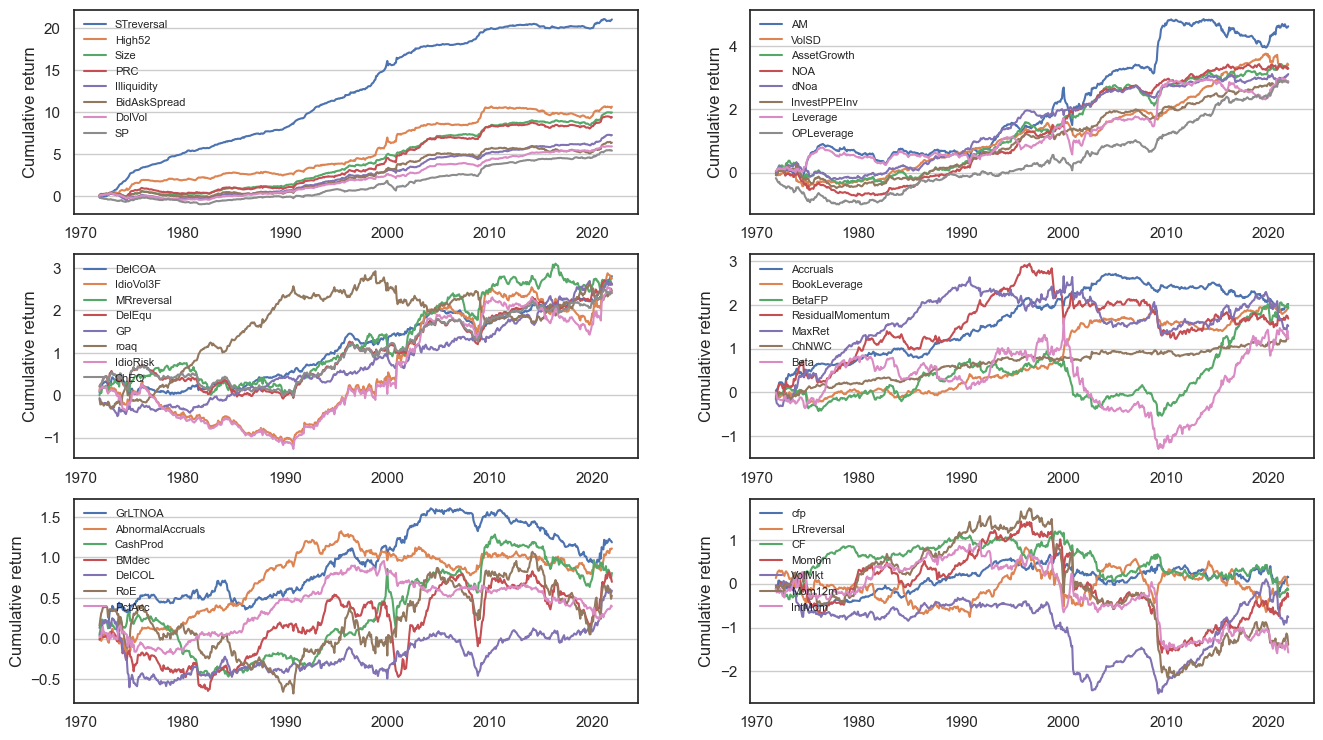
\includegraphics[width=.8\textwidth]{images/univariate_ls_cum_ret_ff5.png}
  \label{fig: ff5 univariate ls cumulative return}
  \caption*{\footnotesize{This graphic showcases firm characteristics sorted univariate long-short portfolios' cumulative return acrossing the whole time period, the return refering to the abnormal return derived from FF5 factor model.}}
\end{figure}

Table \ref{table: ff5 univariate ls portfolio} reports the Sharpe ratio and mean abnormal return of the firm characteristic sorted univariate long-short portfolios with respect to the stock abnormal return derived from the FF5 factors model. For robustness analysis targeting other measures of stock returns, refer to Appendix \ref{sec:appendixb1}. The first two columns present the portfolios' Sharpe ratio and mean abnormal return in the full sample. The majority of long-short portfolios achieve a Sharpe ratio greater than 0.02 and a mean abnormal return exceeding 0.1\% on a monthly average. In comparison with the market performance, the equal weighted portfolio's Sharpe ratio is 0.016 with a mean abnormal return of 0.098\%, while the value-weighted portfolio's Sharpe ratio is 0.01 with a mean return of 0.052\%. These results suggest that most of the firm characteristics possess predictive power for stock abnormal returns, and the formulated long-short portfolios based on those variables outperform the market abnormal return.

\begin{table}[H]
  \centering
  \footnotesize
  \caption{\textbf{FF5 Abnormal Return: Univariate Long-short Portfolios' Returns}}
  \label{table: ff5 univariate ls portfolio}
  \begin{tabular}{lcc|cc|cc|cc}
  \hline
      ~ & \multicolumn{2}{c}{Full Sample} & \multicolumn{2}{c}{Recession} & \multicolumn{2}{c}{Normal} & \multicolumn{2}{c}{Expansion} \\
      ~ & SR & Mean & SR & Mean & SR & Mean & SR & Mean \\ \hline
      STreversal & 0.035 & 0.484 & 0.041 & 0.499 & 0.029 & 0.403 & 0.035 & 0.559 \\
      Size & 0.017 & 0.284 & 0.017 & 0.260 & 0.015 & 0.283 & 0.018 & 0.313 \\ 
      Illiquidity & 0.012 & 0.237 & 0.010 & 0.175 & 0.012 & 0.281 & 0.014 & 0.284 \\ 
      DolVol & 0.010 & 0.224 & 0.008 & 0.164 & 0.010 & 0.245 & 0.012 & 0.280 \\ 
      High52 & 0.018 & 0.215 & 0.024 & 0.249 & 0.011 & 0.136 & 0.017 & 0.257 \\ 
      PRC & 0.016 & 0.213 & 0.022 & 0.253 & 0.010 & 0.158 & 0.014 & 0.216 \\ 
      SP & 0.009 & 0.174 & 0.011 & 0.165 & 0.008 & 0.195 & 0.008 & 0.185 \\ 
      BidAskSpread & 0.011 & 0.164 & 0.013 & 0.175 & 0.006 & 0.103 & 0.013 & 0.203 \\ 
      NOA & 0.005 & 0.159 & 0.010 & 0.255 & 0.002 & 0.070 & 0.004 & 0.120 \\ 
      VolSD & 0.006 & 0.159 & 0.002 & 0.038 & 0.010 & 0.361 & 0.006 & 0.175 \\ 
      dNoa & 0.005 & 0.158 & 0.007 & 0.217 & 0.002 & 0.057 & 0.006 & 0.183 \\ 
      InvestPPEInv & 0.005 & 0.150 & 0.006 & 0.157 & 0.004 & 0.132 & 0.005 & 0.158 \\ 
      DelCOA & 0.005 & 0.144 & 0.005 & 0.146 & 0.001 & 0.028 & 0.008 & 0.229 \\ 
      AssetGrowth & 0.006 & 0.137 & 0.007 & 0.155 & 0.004 & 0.115 & 0.005 & 0.137 \\ 
      AM & 0.008 & 0.134 & 0.011 & 0.144 & 0.003 & 0.067 & 0.009 & 0.195 \\ 
      OPLeverage & 0.005 & 0.127 & 0.007 & 0.179 & 0.005 & 0.170 & 0.002 & 0.040 \\ 
      Accruals & 0.003 & 0.118 & 0.005 & 0.162 & 0.000 & -0.006 & 0.005 & 0.172 \\ 
      GP & 0.004 & 0.115 & 0.003 & 0.078 & 0.008 & 0.213 & 0.002 & 0.063 \\ 
      BookLeverage & 0.003 & 0.112 & 0.002 & 0.064 & 0.007 & 0.289 & 0.001 & 0.042 \\ 
      DelEqu & 0.004 & 0.104 & 0.008 & 0.171 & 0.001 & 0.015 & 0.004 & 0.105 \\ 
      ChEQ & 0.004 & 0.100 & 0.008 & 0.166 & -0.001 & -0.031 & 0.005 & 0.128 \\ 
      Leverage & 0.005 & 0.093 & 0.007 & 0.095 & 0.000 & 0.012 & 0.007 & 0.180 \\ 
      ChNWC & 0.002 & 0.092 & 0.004 & 0.185 & 0.000 & 0.013 & 0.001 & 0.060 \\ 
      roaq & 0.004 & 0.083 & -0.001 & -0.023 & 0.011 & 0.223 & 0.004 & 0.084 \\ 
      MRreversal & 0.004 & 0.080 & 0.007 & 0.116 & 0.000 & 0.002 & 0.005 & 0.114 \\ 
      AbnormalAccruals & 0.002 & 0.074 & 0.005 & 0.166 & -0.002 & -0.104 & 0.003 & 0.110 \\ 
      GrLTNOA & 0.002 & 0.073 & 0.002 & 0.096 & -0.001 & -0.037 & 0.004 & 0.140 \\ 
      IdioVol3F & 0.005 & 0.072 & 0.008 & 0.105 & 0.001 & 0.017 & 0.004 & 0.079 \\ 
      BetaFP & 0.003 & 0.069 & -0.003 & -0.049 & 0.009 & 0.230 & 0.004 & 0.112 \\ 
      IdioRisk & 0.004 & 0.065 & 0.008 & 0.107 & 0.000 & 0.003 & 0.004 & 0.065 \\ 
      ResidualMomentum & 0.003 & 0.051 & 0.002 & 0.030 & 0.001 & 0.017 & 0.006 & 0.104 \\ 
      MaxRet & 0.003 & 0.045 & 0.000 & 0.006 & 0.005 & 0.091 & 0.003 & 0.055 \\ 
      CashProd & 0.001 & 0.039 & 0.000 & -0.011 & 0.000 & 0.008 & 0.004 & 0.145 \\ 
      DelCOL & 0.001 & 0.034 & 0.000 & 0.006 & 0.000 & 0.004 & 0.003 & 0.091 \\ 
      BMdec & 0.001 & 0.029 & -0.004 & -0.082 & 0.001 & 0.018 & 0.007 & 0.198 \\ 
      Beta & 0.002 & 0.029 & -0.002 & -0.031 & 0.010 & 0.139 & 0.000 & -0.004 \\ 
      PctAcc & 0.001 & 0.027 & 0.000 & 0.003 & -0.001 & -0.041 & 0.002 & 0.098 \\ 
      RoE & 0.001 & 0.017 & 0.007 & 0.127 & -0.005 & -0.107 & 0.000 & 0.000 \\ 
      cfp & 0.000 & 0.006 & -0.002 & -0.052 & 0.002 & 0.050 & 0.002 & 0.038 \\ 
      LRreversal & 0.000 & -0.001 & 0.006 & 0.100 & -0.007 & -0.111 & -0.001 & -0.009 \\ 
      CF & 0.000 & -0.005 & -0.004 & -0.074 & 0.002 & 0.061 & 0.001 & 0.022 \\ 
      Mom6m & 0.000 & -0.007 & -0.002 & -0.029 & 0.001 & 0.015 & 0.000 & 0.001 \\ 
      VolMkt & -0.001 & -0.023 & -0.008 & -0.118 & 0.005 & 0.117 & 0.000 & 0.009 \\ 
      Mom12m & -0.002 & -0.030 & -0.008 & -0.086 & 0.003 & 0.043 & -0.002 & -0.025 \\ 
      IntMom & -0.003 & -0.041 & -0.007 & -0.090 & 0.001 & 0.022 & -0.002 & -0.037 \\ \hline
  \end{tabular}
  \begin{tablenotes}
    \footnotesize
    \item This table presents firm characteristics sorted univariate long-short portfolios' sharpe ratios and mean returns. The dataset has futher splitted into three different subsamples based on macroeconomic condition indicator -- CFNAI index, named by recession, normal, and expansion period. The return in this table refering to the abnormal stock return derived from FF5 factors model.
  \end{tablenotes}
\end{table}

Next, we study the performance of univariate long-short portfolios in different macroeconomic conditions. The construction of CFNAI index indicating that a positive index reading corresponds to growth above trend and a negative index reading corresponds to growth below trend. Based on CFNAI we sort the data into tertiles, and define those tertiles from top to bottom as expansion, normal, and recession period. In Table \ref{table: ff5 univariate ls portfolio}, columns 3-8 report univariate long-short portfolios' Sharpe ratios and mean abnormal returns across different macroeconomic conditions. The result of comparing those figures horizontally across 3 macroeconomic senarios as presented in Figure \ref{fig: ff5 univariate ls comparing}. 

The left panel of the figure presents the portfolios' Sharpe ratio under different macroeconomic conditions. The frequency of recession and expansion periods ranked in the 1st and 2nd places is higher than that in the 3rd place, indicating that during both recession and expansion periods, the portfolios tend to have higher Sharpe ratios than in normal periods. We observe a similar pattern in the right panel when considering the portfolios' mean return. Based on these results, we can preliminarily conclude that during recession and expansion periods, the Fama-French 5 factor model's predicted return deviates the most from the actual realized stock return, while in normal periods, when the market is less volatile, the model's predicted return deviates the least. Evidently, there exists an interaction effect between stock abnormal return and macroeconomic conditions.

\begin{figure}[H]
  \centering
  \caption{\textbf{FF5 Abnormal Return: Univariate Long-short Portfolios Performance in Different Macroeconomic Conditions}}
  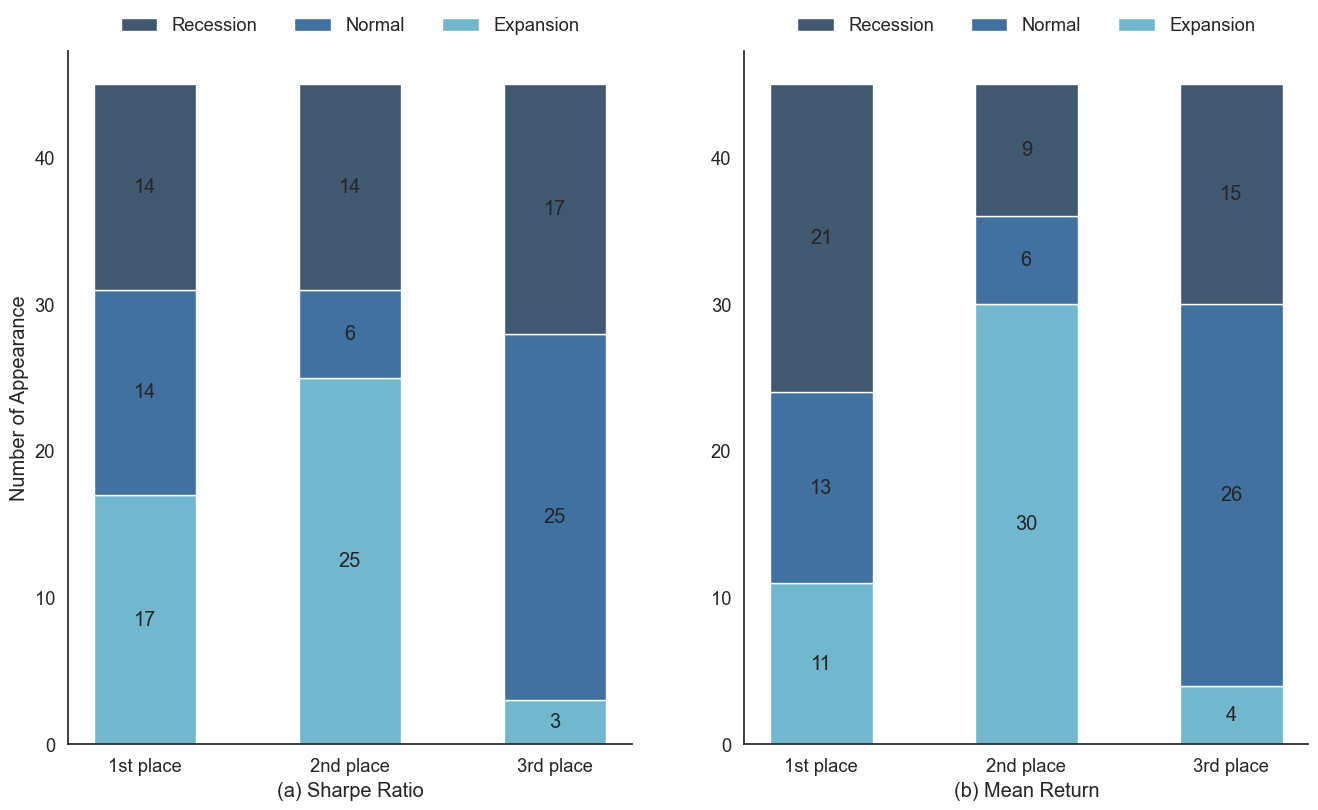
\includegraphics[width=.8\textwidth]{images/univariant_ls_ff5_comparing.png}
  \label{fig: ff5 univariate ls comparing}
  \caption*{\footnotesize{This graphic showcases firm characteristics sorted long-short univariate portfolios' performance across different macroeconomic conditions. We compare univariate long-short portfolios' sharpe ratio and mean return in recession, normal, and expansion periods, which is the horizontal comparision among the last 6 columns in table \ref{table: ff5 univariate ls portfolio}.}}
\end{figure}